\documentclass[conference]{IEEEtran}
\IEEEoverridecommandlockouts
\usepackage{cite}
\usepackage{amsmath,amssymb,amsfonts}
\usepackage{algorithmic}
\usepackage{algorithm}
\usepackage{graphicx}
\usepackage{textcomp}
\usepackage{xcolor}
\usepackage{booktabs}
\usepackage{multirow}
\usepackage{hyperref}
\usepackage{subcaption}
\usepackage{float}
\usepackage{tikz}
\usetikzlibrary{shapes.geometric, arrows.meta, positioning, fit, calc}

\graphicspath{{../models/}}

\def\BibTeX{{\rm B\kern-.05em{\sc i\kern-.025em b}\kern-.08em
    T\kern-.1667em\lower.7ex\hbox{E}\kern-.125emX}}

\begin{document}

\title{When Scheduling Fails: Batched Execution in LLM Systems}

\author{
\IEEEauthorblockN{Muaaz Shaikh*}
\IEEEauthorblockA{\textit{B.Tech CSBS} \\
\textit{MPSTME, NMIMS University}\\
Mumbai, India \\
muaaz5731@gmail.com}
\and
\IEEEauthorblockN{Dhruvil Parekh}
\IEEEauthorblockA{\textit{B.Tech CSBS} \\
\textit{MPSTME, NMIMS University}\\
Mumbai, India \\
dhruvilparekh726@gmail.com}
\and
\IEEEauthorblockN{Vaishnavi Parashar}
\IEEEauthorblockA{\textit{B.Tech CSBS} \\
\textit{MPSTME, NMIMS University}\\
Mumbai, India \\
vaishnaviparashar2006@gmail.com}
\and
\IEEEauthorblockN{Swarnalata Bollavarapu}
\IEEEauthorblockA{\textit{Department Of Computer Engineering} \\
\textit{MPSTME, NMIMS University}\\
Mumbai, India \\
Swarnalata.B@nmims.edu}
}

\maketitle

% ============================================================
\begin{abstract}
% ============================================================
Classical OS scheduling theory assumes that job sizes are observable and execution is sequential, enabling algorithms like Shortest Job First (SJF) to provably minimize average waiting time. LLM agent operating systems such as AIOS~\cite{mei2025aios} introduce a fundamentally different execution model: requests are batched to a GPU, actual output length is unobservable a priori, and batch-level dynamics dominate individual request latency. To our knowledge, we present the first empirical study examining whether these differences invalidate classical scheduling assumptions. We instrument the AIOS kernel to log 15 per-syscall features, collect 2,000 syscalls across two LLM backends (Llama~3.1:8b and Mistral:7b) with five concurrent agent types, and conduct a three-phase investigation: (1)~feature-latency correlation analysis revealing that request properties are weak predictors (max Spearman $\rho = 0.206$); (2)~a six-model ML classification study achieving F1~=~0.47, confirming that latency classes are not separable from input features; and (3)~a simulation of 16~classical scheduling algorithms demonstrating that FIFO matches or outperforms all alternatives on average turnaround. We identify the root cause: GPU batching destroys the job-size observability assumption that underpins SJF optimality. However, we show that SJF and Priority scheduling reduce fast-task wait time by 68--73\% at the cost of large-task degradation, revealing a fairness-latency tradeoff absent from the original AIOS design. We release six integrated scheduler implementations and a simulation framework for AIOS.
\end{abstract}

\begin{IEEEkeywords}
LLM agents, operating systems, scheduling algorithms, AIOS, GPU batching, job-size observability
\end{IEEEkeywords}

% ============================================================
\section{Introduction}
% ============================================================

The deployment of LLM-based autonomous agents~\cite{yao2023react, shinn2023reflexion} has motivated OS-level abstractions for managing concurrent access to shared LLM resources. AIOS~\cite{mei2025aios} introduces such an abstraction: agent queries are decomposed into typed system calls (LLM, memory, storage, tool) and dispatched by a centralized scheduler. The original architecture provides FIFO and Round Robin scheduling, achieving up to 2.1$\times$ throughput over unscheduled frameworks~\cite{mei2025aios}.

A natural next step is to apply classical scheduling theory to this new domain. In traditional OS scheduling, Shortest Job First (SJF) provably minimizes average waiting time when job sizes are known~\cite{silberschatz2018os}. LLM requests carry rich metadata---prompt length, token budget, conversation depth---that might serve as job-size proxies. This motivates our central research question:

\begin{quote}
\textit{Do classical OS scheduling assumptions---observable job sizes and sequential execution---hold in LLM agent systems? If not, what are the implications for scheduler design?}
\end{quote}

We hypothesize that request-level features can approximate job size, enabling classical scheduling improvements over FIFO. We test this hypothesis through three progressively refined approaches and ultimately \textit{reject} it, providing a structural explanation rooted in GPU batch execution dynamics. While prior work establishes the need for scheduling in LLM agent systems~\cite{mei2025aios}, our results reveal a fundamental limitation: \textit{under GPU batching, request-level scheduling provides negligible benefit over FIFO}.

\smallskip
\noindent\textbf{Contributions.} Our work provides:

\begin{enumerate}
    \item \textbf{Empirical evidence} that request-level features are weak latency predictors ($\rho \leq 0.206$) for batched single-GPU LLM inference, due to GPU batching destroying job-size observability.
    \item A \textbf{system-level identification} of two violated assumptions: (a) job sizes are not estimable from input features because \texttt{max\_tokens} is a ceiling, not a target, and (b) execution is batched, not sequential, nullifying SJF's optimality proof.
    \item \textbf{Quantitative evidence} that FIFO is near-optimal under GPU batching constraints, outperforming all 16 simulated classical algorithms on average turnaround.
    \item \textbf{Discovery of a fairness--latency tradeoff}: SJF reduces fast-task wait by 68\% while increasing large-task wait by 94\%, a dimension absent from the original AIOS scheduler design.
    \item \textbf{Open-source release} of six scheduler implementations (FIFO, SJF, Priority, MLFQ, HRRN, ML-based) and a simulation framework integrated into AIOS.
\end{enumerate}

% ============================================================
\section{Related Work}
% ============================================================

\textbf{LLM Agent Operating Systems.}
AIOS~\cite{mei2025aios} provides the foundational architecture, with Cerebrum~\cite{rama2025cerebrum} extending it as an SDK. MemGPT~\cite{packer2023memgpt} proposes LLM-as-OS with virtual memory. None of these works investigate request-aware scheduling policies.

\textbf{OS Scheduling Theory.}
SJF minimizes average waiting time for non-preemptive scheduling when job sizes are known~\cite{liu1973scheduling}. MLFQ provides adaptive scheduling without advance knowledge~\cite{corbato1962experimental}. HRRN balances responsiveness with starvation prevention~\cite{silberschatz2018os}. These algorithms assume sequential execution and observable job sizes---assumptions we test empirically.

\textbf{ML for Systems.}
Learned scheduling has been applied in databases~\cite{kraska2018case}, clusters~\cite{mao2019learning}, and compilers~\cite{chen2018tvm}. In LLM inference, FlexGen~\cite{sheng2023flexgen} optimizes throughput for single-GPU serving. Our work is the first to apply ML-based scheduling within an LLM agent OS.

% ============================================================
\section{System Architecture and Methodology}
% ============================================================

\subsection{AIOS Scheduling Pipeline}

Fig.~\ref{fig:architecture} illustrates our instrumented scheduling pipeline within AIOS. Agent applications submit queries through the AIOS SDK, which decomposes them into typed system calls. LLM syscalls enter a global request queue, where the scheduler selects a batch for dispatch to the Ollama LLM backend. Our instrumentation logs 15 features per syscall at completion (Table~\ref{tab:features}).

\begin{figure}[htbp]
\centering
\resizebox{0.98\columnwidth}{!}{%
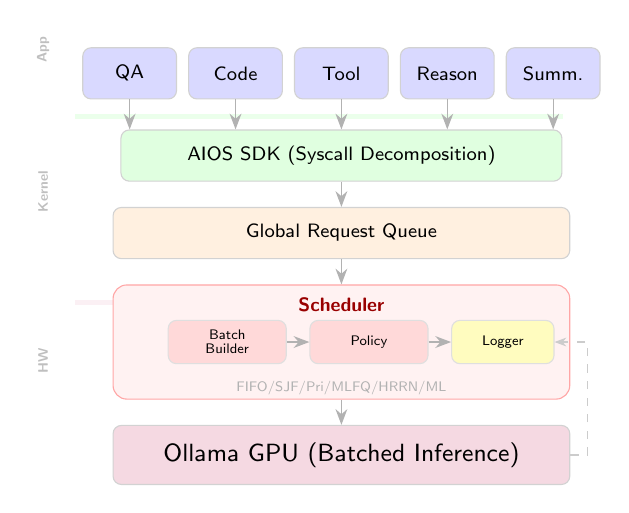
\begin{tikzpicture}[
    node distance=0.4cm and 0.15cm,
    box/.style={rectangle, draw=gray!35, rounded corners=3pt, minimum height=0.65cm, font=\scriptsize\sffamily, align=center, fill=#1, text width=1.05cm, inner sep=2pt},
    wide/.style={rectangle, draw=gray!35, rounded corners=3pt, minimum height=0.65cm, font=\scriptsize\sffamily, align=center, fill=#1, inner sep=4pt},
    sched/.style={rectangle, draw=red!35, rounded corners=5pt, fill=red!5, inner sep=6pt},
    schedbox/.style={rectangle, draw=gray!25, rounded corners=3pt, minimum height=0.55cm, font=\tiny\sffamily, align=center, fill=#1, inner sep=3pt},
    arrow/.style={-{Stealth[length=2mm, width=1.5mm]}, gray!60, line width=0.6pt},
    lbl/.style={font=\tiny\sffamily\bfseries, color=gray!50}
]

% ---- Layer labels ----
\node[lbl, rotate=90] at (-1.1, 0.3) {App};
\node[lbl, rotate=90] at (-1.1, -1.5) {Kernel};
\node[lbl, rotate=90] at (-1.1, -3.65) {HW};

% ---- Layer separators ----
\fill[green!8] (-0.7, -0.52) rectangle (5.5, -0.58);
\fill[purple!6] (-0.7, -2.88) rectangle (5.5, -2.94);

% ---- App layer: Agent boxes ----
\node[box=blue!15] (a1) {QA};
\node[box=blue!15, right=0.14cm of a1] (a2) {Code};
\node[box=blue!15, right=0.14cm of a2] (a3) {Tool};
\node[box=blue!15, right=0.14cm of a3] (a4) {Reason};
\node[box=blue!15, right=0.14cm of a4] (a5) {Summ.};

% ---- Kernel layer ----
\node[wide=green!12, below=0.38cm of a3, minimum width=5.6cm] (sdk) {AIOS SDK (Syscall Decomposition)};

\node[wide=orange!12, below=0.32cm of sdk, minimum width=5.8cm] (queue) {Global Request Queue};

% ---- Scheduler container ----
\node[sched, below=0.32cm of queue, minimum width=5.8cm, minimum height=1.45cm] (schedcontainer) {};
\node[font=\scriptsize\sffamily\bfseries, color=red!60!black] at (schedcontainer.north) [below=0.05cm] {Scheduler};

% Scheduler internals
\node[schedbox=red!15, minimum width=1.5cm] at ($(schedcontainer.center)+(-1.45, 0.0)$) (batcher) {Batch\\[-1pt]Builder};
\node[schedbox=red!15, minimum width=1.5cm] at ($(schedcontainer.center)+(0.35, 0.0)$) (policy) {Policy};
\node[schedbox=yellow!25, minimum width=1.3cm] at ($(schedcontainer.center)+(2.05, 0.0)$) (logger) {Logger};

\draw[arrow] (batcher) -- (policy);
\draw[arrow] (policy) -- (logger);

% Policy label
\node[font=\tiny\sffamily, color=gray!60] at ($(schedcontainer.south)+(0, 0.15)$) {FIFO/SJF/Pri/MLFQ/HRRN/ML};

% ---- HW layer ----
\node[wide=purple!15, below=0.32cm of schedcontainer, minimum width=5.8cm, minimum height=0.75cm, font=\small\sffamily] (llm) {Ollama GPU (Batched Inference)};

% ---- Connecting arrows ----
\foreach \a in {a1,a2,a3,a4,a5}
    \draw[arrow, line width=0.45pt] (\a) -- (\a |- sdk.north);
\draw[arrow] (sdk) -- (queue);
\draw[arrow] (queue) -- (schedcontainer.north);
\draw[arrow] (schedcontainer.south) -- (llm.north);

% Feedback arrow
\draw[-{Stealth[length=1.5mm]}, gray!40, line width=0.4pt, dashed] (llm.east) -- ++(0.22,0) |- (logger.east);

\end{tikzpicture}%
}
\caption{Instrumented AIOS scheduling pipeline. The kernel layer shows the scheduler internals: batch collection, policy-based ordering, and logging. Dashed arrow shows completion feedback.}
\label{fig:architecture}
\end{figure}

\begin{table}[htbp]
\caption{Logged Syscall Features (15 per request)}
\begin{center}
\begin{tabular}{llp{3.2cm}}
\toprule
\textbf{Category} & \textbf{Feature} & \textbf{Description} \\
\midrule
\multirow{5}{*}{Request} & \texttt{input\_char\_length} & Total prompt character count \\
& \texttt{message\_count} & Conversation turns (2--8) \\
& \texttt{has\_tools} & Tool schema attached \\
& \texttt{max\_tokens} & Generation budget ceiling \\
& \texttt{temperature} & Sampling temperature \\
\midrule
\multirow{2}{*}{Context} & \texttt{model\_name} & LLM backend identifier \\
& \texttt{agent\_name} & Agent type + round \\
\midrule
\multirow{4}{*}{Timing} & \texttt{created\_time} & Queue arrival \\
& \texttt{start\_time} & Execution start \\
& \texttt{end\_time} & Execution end \\
& \texttt{latency\_ms} & $\text{end} - \text{start}$ \\
\midrule
\multirow{3}{*}{Outcome} & \texttt{wait\_ms} & $\text{start} - \text{created}$ \\
& \texttt{was\_interrupted} & Context switch occurred \\
& \texttt{error} & Error flag \\
\bottomrule
\end{tabular}
\label{tab:features}
\end{center}
\end{table}

\subsection{Experiment Pipeline}

Fig.~\ref{fig:pipeline} shows our three-phase investigation methodology.

\begin{figure}[htbp]
\centering
\resizebox{\columnwidth}{!}{%
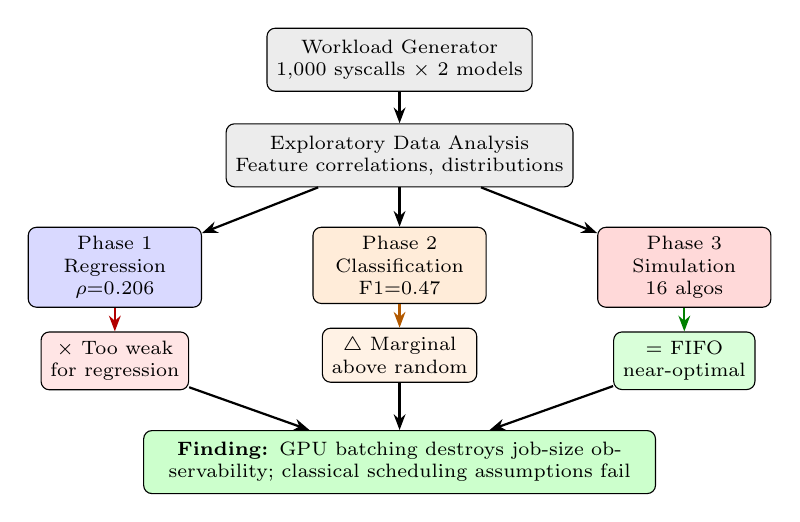
\begin{tikzpicture}[
    node distance=0.3cm and 0.3cm,
    phase/.style={rectangle, draw, rounded corners=3pt, minimum height=0.8cm, minimum width=2.2cm, font=\scriptsize, align=center, fill=#1},
    result/.style={rectangle, draw, rounded corners=3pt, minimum height=0.6cm, font=\scriptsize, align=center, fill=#1, minimum width=1.3cm},
    arrow/.style={-{Stealth[length=2mm]}, thick},
    xarrow/.style={-{Stealth[length=2mm]}, thick, color=red!70!black},
]
% Data
\node[phase=gray!15] (collect) {Workload Generator\\1,000 syscalls $\times$ 2 models};
\node[phase=gray!15, below=0.4cm of collect] (eda) {Exploratory Data Analysis\\Feature correlations, distributions};

% Three phases side by side
\node[phase=blue!15, below left=0.5cm and 0.3cm of eda] (reg) {Phase 1\\Regression\\$\rho{=}0.206$};
\node[phase=orange!15, below=0.5cm of eda] (cls) {Phase 2\\Classification\\F1${=}$0.47};
\node[phase=red!15, below right=0.5cm and 0.3cm of eda] (sim) {Phase 3\\Simulation\\16 algos};

% Results
\node[result=red!10, below=0.3cm of reg] (r1) {$\times$ Too weak\\for regression};
\node[result=orange!10, below=0.3cm of cls] (r2) {$\triangle$ Marginal\\above random};
\node[result=green!15, below=0.3cm of sim] (r3) {$=$ FIFO\\near-optimal};

% Final
\node[phase=green!20, below=0.6cm of r2, minimum width=6.5cm, text width=6cm] (finding) {\textbf{Finding:} GPU batching destroys job-size observability; classical scheduling assumptions fail};

\draw[arrow] (collect) -- (eda);
\draw[arrow] (eda) -- (reg);
\draw[arrow] (eda) -- (cls);
\draw[arrow] (eda) -- (sim);
\draw[xarrow] (reg) -- (r1);
\draw[arrow, color=orange!70!black] (cls) -- (r2);
\draw[arrow, color=green!50!black] (sim) -- (r3);
\draw[arrow] (r1) -- (finding);
\draw[arrow] (r2) -- (finding);
\draw[arrow] (r3) -- (finding);

\end{tikzpicture}%
}
\caption{Three-phase experiment pipeline. Each phase independently converges on the same conclusion: request features cannot predict latency under GPU-batched execution.}
\label{fig:pipeline}
\end{figure}

\subsection{Workload Design}
To avoid confounding agent type with request configuration (a limitation of the original AIOS benchmarks, where each agent has fixed \texttt{max\_tokens} and \texttt{temperature}), we randomize all parameters independently:

\begin{itemize}
    \item \textbf{max\_tokens}: Uniform from \{64, 128, 256, 512, 1024, 2048\}
    \item \textbf{temperature}: Uniform from \{0.1, 0.2, 0.3, 0.5, 0.7, 0.9, 1.0\}
    \item \textbf{Multi-turn}: 30\% of requests include 1--3 follow-up exchanges
    \item \textbf{Prompt padding}: 30\% receive a long prefix ($\sim$400 chars); 20\% receive a short suffix
    \item \textbf{Arrival stagger}: Random 1--5s sleep between requests
\end{itemize}

Five agent types (short\_qa, long\_reasoning, tool\_use, code\_gen, summarizer) run concurrently across 20 rounds per model, yielding 1,000 syscalls per LLM backend.

% ============================================================
\section{Experimental Setup}
% ============================================================

\textbf{Inference backend:} Single Ollama~\cite{ollama} instance serving one model at a time.

\textbf{Models:} Llama 3.1:8b~\cite{dubey2024llama} (8B params) and Mistral:7b~\cite{jiang2023mistral} (7B params), both instruction-tuned, running locally.

\textbf{Dataset:} 2,000 syscalls (1,000 per model) with zero errors and zero interruptions. Table~\ref{tab:dataset} summarizes the combined statistics.

\begin{table}[htbp]
\caption{Combined Dataset Statistics (N = 2,000)}
\begin{center}
\begin{tabular}{lrrrrr}
\toprule
\textbf{Feature} & \textbf{Mean} & \textbf{Std} & \textbf{Median} & \textbf{Min} & \textbf{Max} \\
\midrule
latency\_ms & 5,932 & 3,642 & 5,205 & 22 & 21,484 \\
wait\_ms & 1,810 & 2,380 & 910 & 103 & 16,196 \\
char\_length & 880 & 680 & 580 & 165 & 2,658 \\
msg\_count & 3.0 & 2.1 & 2 & 2 & 8 \\
max\_tokens & 684 & 660 & 512 & 64 & 2,048 \\
\bottomrule
\end{tabular}
\label{tab:dataset}
\end{center}
\end{table}

\textbf{Dataset justification.} While 2,000 samples is modest for general ML, our setting is a controlled experiment with exhaustive parameter randomization across a fixed set of 5 agent types, 6 token budgets, 7 temperatures, and 2 models. Each configuration appears multiple times, providing sufficient coverage for the correlation and classification analyses. We validate all results with stratified 5-fold cross-validation and report confidence intervals where applicable.

% ============================================================
\section{Phase 1: Feature-Latency Analysis}
% ============================================================

\subsection{Hypothesis}
We hypothesize that request-level features---particularly \texttt{max\_tokens} and \texttt{input\_char\_length}---correlate with latency strongly enough to enable predictive scheduling.

\subsection{Results}
Table~\ref{tab:correlations} reports Spearman rank correlations. The strongest predictor is \texttt{max\_tokens} ($\rho = 0.206$, $p < 10^{-20}$). All other features have $|\rho| < 0.05$ with latency. Fig.~\ref{fig:model_comparison} shows the latency distributions for both models.

\begin{table}[htbp]
\caption{Feature-Latency Spearman Correlations (N = 2,000)}
\begin{center}
\begin{tabular}{lrrl}
\toprule
\textbf{Feature} & \textbf{$\rho$} & \textbf{$p$-value} & \textbf{Interpretation} \\
\midrule
max\_tokens & 0.206 & $1.5 \times 10^{-20}$ & Weak positive \\
model\_name & 0.132 & $3.2 \times 10^{-9}$ & Llama slower \\
input\_char\_length & 0.049 & $2.9 \times 10^{-2}$ & Negligible \\
temperature & 0.031 & $1.7 \times 10^{-1}$ & Not significant \\
message\_count & $-0.013$ & $5.7 \times 10^{-1}$ & Not significant \\
\bottomrule
\end{tabular}
\label{tab:correlations}
\end{center}
\end{table}

\begin{figure}[htbp]
\centerline{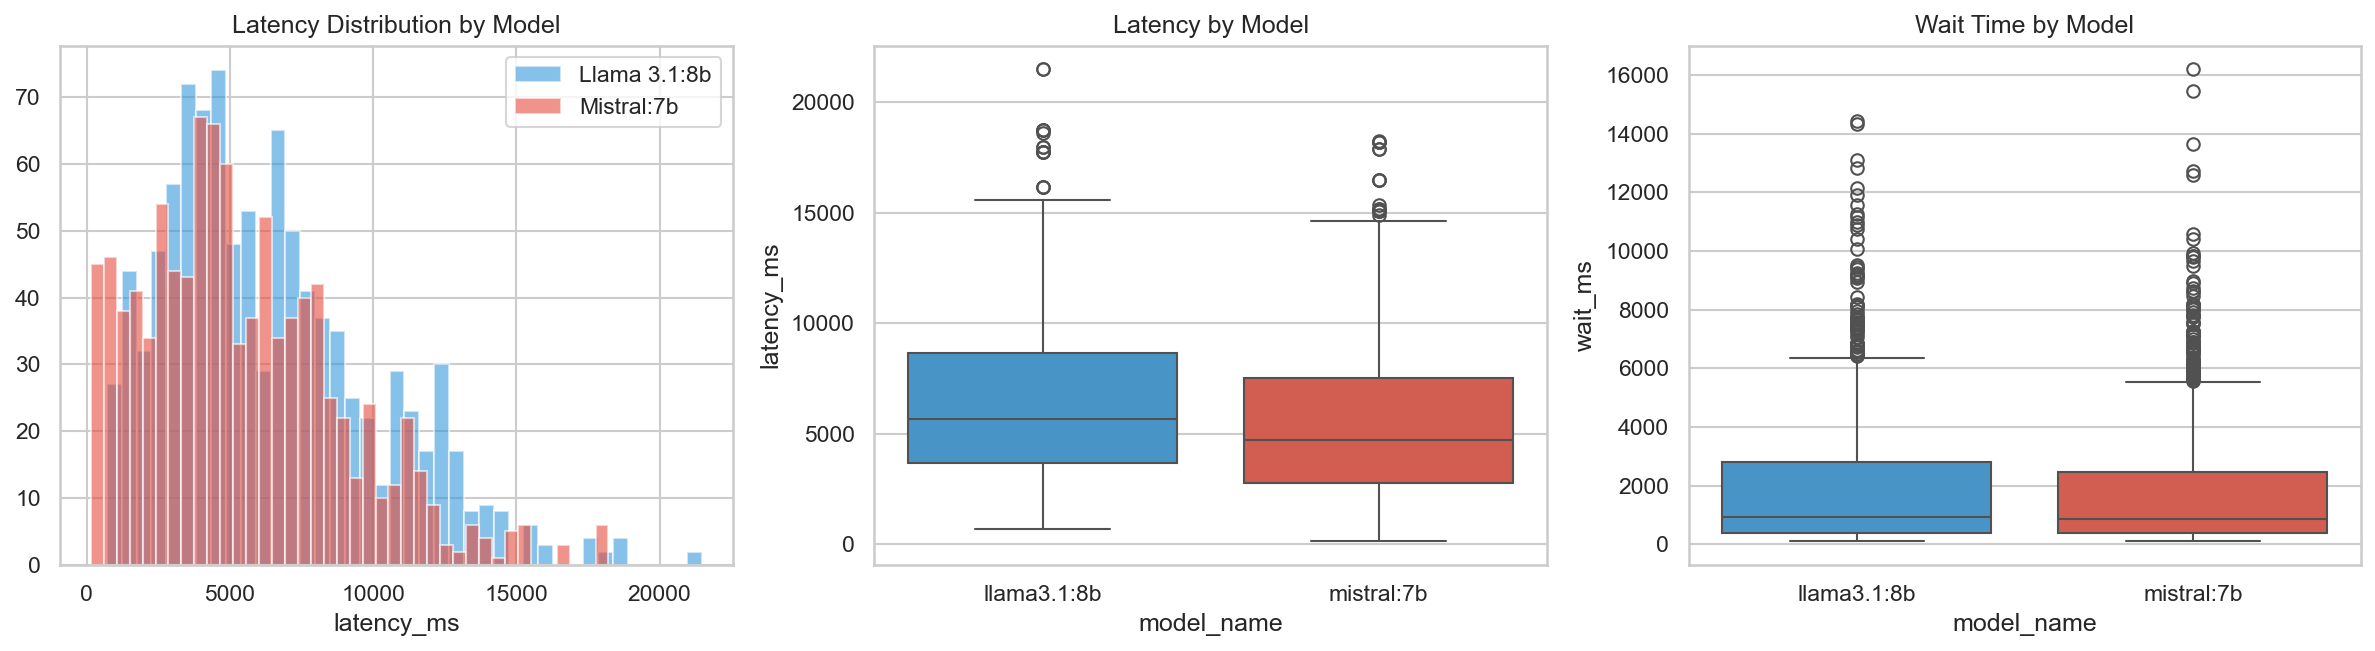
\includegraphics[width=\columnwidth]{model_comparison_latency.png}}
\caption{Latency distributions for Llama 3.1:8b (median 5,657ms) and Mistral:7b (median 4,738ms). Llama is consistently 920ms slower despite similar parameter count.}
\label{fig:model_comparison}
\end{figure}

\subsection{Structural Explanation: Why Features Fail}

The weak correlations have a \textit{structural} explanation rooted in how LLM inference works:

\begin{enumerate}
    \item \textbf{max\_tokens is a ceiling, not a target.} The model generates until it emits an end-of-sequence (EOS) token \textit{or} reaches \texttt{max\_tokens}. In practice, the model stops early for most requests. Setting \texttt{max\_tokens}=2048 does not produce 2048 tokens. Only low values (64, 128) actively truncate output, creating the observed weak positive correlation.

    \item \textbf{GPU batching decouples individual latency from request properties.} Ollama batches concurrent requests to the GPU. All requests in a batch complete at approximately the same time regardless of individual \texttt{max\_tokens} or prompt length, because the GPU processes prefill in parallel and decode steps are dominated by the longest-generating request in the batch.

    \item \textbf{Actual output length is unobservable a priori.} The true latency driver is how many tokens the model \textit{actually generates}, which depends on semantic content, not on any input feature. This is the fundamental difference from classical OS scheduling, where job size is observable.
\end{enumerate}

\begin{figure}[htbp]
\centerline{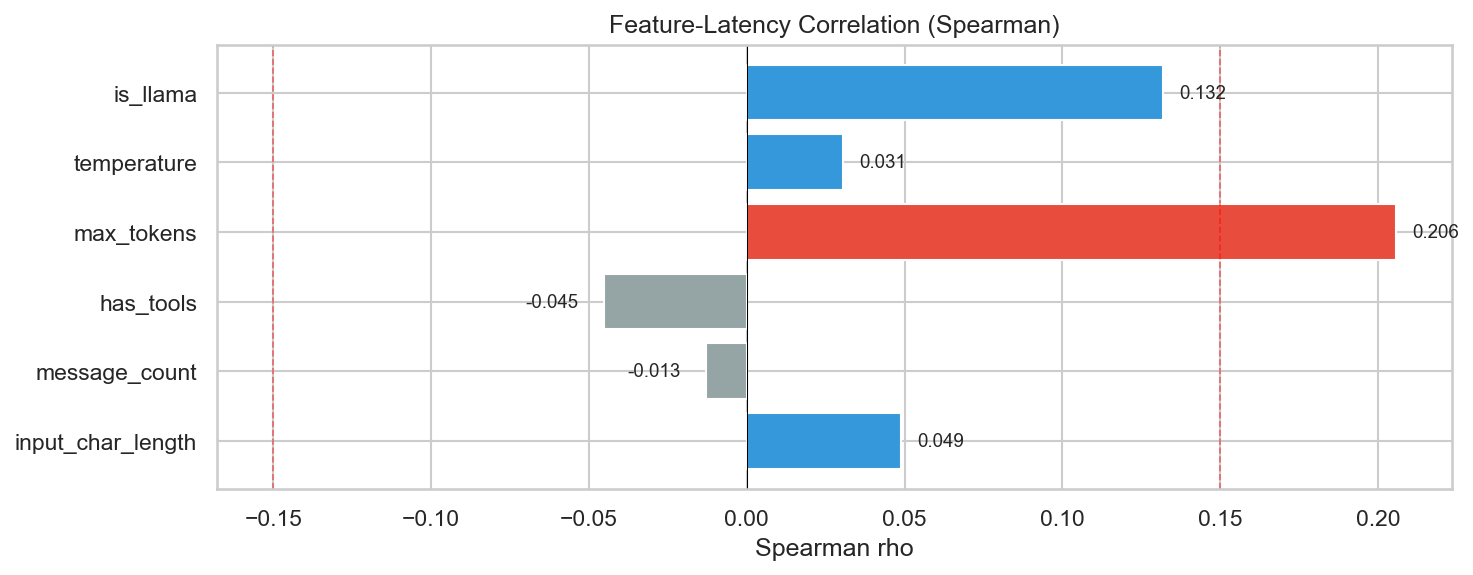
\includegraphics[width=\columnwidth]{correlation_bars.png}}
\caption{Spearman correlation of each feature with latency. Only \texttt{max\_tokens} exceeds $|\rho| = 0.1$. Dashed red lines indicate $|\rho| = 0.15$ threshold.}
\label{fig:correlations}
\end{figure}

\subsection{Conclusion}
\textbf{Hypothesis rejected.} Request features are insufficient for predictive scheduling (Approach 1 / Cognitive Scheduler). This is a \textit{negative result with structural explanation}: the failure is not due to insufficient data or poor modeling, but due to a fundamental mismatch between the scheduling assumption (observable job sizes) and the execution model (GPU-batched inference with unobservable output length).

% ============================================================
\section{Phase 2: Classification-Based Scheduling}
% ============================================================

Since continuous prediction failed, we attempted discrete classification into priority classes.

\subsection{Setup}
We define three classes using percentile thresholds: \texttt{fast} ($< p_{33} = 3,846$ms), \texttt{medium} ($p_{33}$--$p_{66}$), \texttt{large} ($\geq p_{66} = 6,993$ms). The feature vector includes 5 numeric features, 5 agent-type one-hot indicators, and 2 model indicators (12 features total). We evaluate six classifiers with stratified 5-fold CV on 80\% of the data.

\subsection{Results}

\begin{table}[htbp]
\caption{Classifier Comparison (Stratified 5-Fold CV, N=1,609)}
\begin{center}
\begin{tabular}{lcccc}
\toprule
\textbf{Model} & \textbf{F1} & \textbf{Acc} & \textbf{Gap} & \textbf{Diagnosis} \\
\midrule
Grad. Boosting & \textbf{0.438} & 0.439 & 0.226 & High bias \\
Random Forest & 0.404 & 0.405 & 0.585 & Overfitting \\
SVM (RBF) & 0.383 & 0.399 & 0.085 & High bias \\
Logistic Reg. & 0.381 & 0.395 & 0.017 & High bias \\
KNN ($k$=5) & 0.378 & 0.397 & 0.181 & High bias \\
Decision Tree & 0.335 & 0.340 & 0.601 & Overfitting \\
\midrule
\multicolumn{2}{l}{\textit{Random baseline}} & \multicolumn{1}{c}{\textit{0.333}} & & \\
\bottomrule
\end{tabular}
\label{tab:classifiers}
\end{center}
\end{table}

After hyperparameter tuning (432-candidate grid search), Gradient Boosting achieves held-out F1 = 0.47 (accuracy 0.47). Feature importances: \texttt{input\_char\_length} (0.36), \texttt{max\_tokens} (0.24), \texttt{agent\_code\_gen} (0.10). The ``medium'' class is poorly discriminated (F1 = 0.41), while ``fast'' (F1 = 0.47) and ``large'' (F1 = 0.52) show partial separability.

\subsection{Analysis: Why Classification is Weak}

The F1 of 0.47 (vs. 0.33 random baseline) represents a 42\% improvement over chance but remains insufficient for reliable scheduling. The root cause is identical to Phase 1: latency classes are defined by \textit{actual execution time}, which depends on batch dynamics and output length, not input features. The classifier learns a noisy approximation of the max\_tokens $\rightarrow$ latency relationship, which is the only signal available.


% ============================================================
\section{Phase 3: Classical Algorithm Simulation}
% ============================================================

\subsection{Methodology}
We simulate 16 scheduling algorithms on the logged data. Syscalls are grouped into batches using a 3-second arrival window (avg batch size: 2.5). Within each batch, the algorithm determines dispatch order. We model sequential execution: each request starts after the previous completes, preserving logged inference times. We compute simulated wait time ($W$) and turnaround time ($T = W + \text{latency}$).

\textbf{Simulation limitation.} We acknowledge that this sequential model does not capture Ollama's parallel GPU batching. Our sequential simulation models batch completion as dominated by the slowest request, capturing the key effect of GPU batching, though it does not simulate parallel kernel execution. Crucially, the sequential model provides an \textit{upper bound} on reordering benefit: since SJF is provably optimal for minimizing average wait under sequential non-preemptive execution~\cite{silberschatz2018os}, any failure to improve over FIFO in this setting implies strictly weaker gains under coupled batch execution where $T_{\text{batch}} = \max(T_i)$.

\subsection{Algorithms}
We evaluate: FIFO, LIFO, SJF (by \texttt{max\_tokens}), LJF, SJF (by \texttt{input\_char\_length}), SRTF (estimated cost), Priority (static rules), HRRN, EDF, Aging SJF, Round Robin, Multi-Level Queue, Fair Share, Lottery, Temp-First, and Combined Score. Full definitions are in the supplementary materials.

\subsection{Overall Results}

Table~\ref{tab:simulation} and Fig.~\ref{fig:simulation} report the results.

\begin{table}[htbp]
\caption{Scheduling Simulation (Top 8 of 16, N=2,000)}
\begin{center}
\begin{tabular}{lrrrr}
\toprule
\textbf{Algorithm} & \textbf{Avg $T$} & \textbf{Med $T$} & \textbf{P95 $T$} & \textbf{vs FIFO} \\
 & \textbf{(ms)} & \textbf{(ms)} & \textbf{(ms)} & \\
\midrule
FIFO & 11,558 & 8,650 & 30,947 & --- \\
Round Robin & 11,558 & 8,650 & 30,947 & 0.0\% \\
Fair Share & 11,558 & 8,650 & 30,947 & 0.0\% \\
EDF & 11,684 & 8,762 & 31,323 & +1.1\% \\
Aging SJF & 11,798 & 8,856 & 31,571 & +2.1\% \\
HRRN & 11,822 & 8,912 & 31,603 & +2.3\% \\
Priority & 12,064 & 9,013 & 32,165 & +4.4\% \\
SJF & 12,269 & 9,251 & 32,763 & +6.2\% \\
\midrule
\textit{LIFO (worst)} & \textit{13,710} & \textit{10,608} & \textit{35,705} & \textit{+18.6\%} \\
\bottomrule
\end{tabular}
\label{tab:simulation}
\end{center}
\end{table}

\begin{figure}[htbp]
\centerline{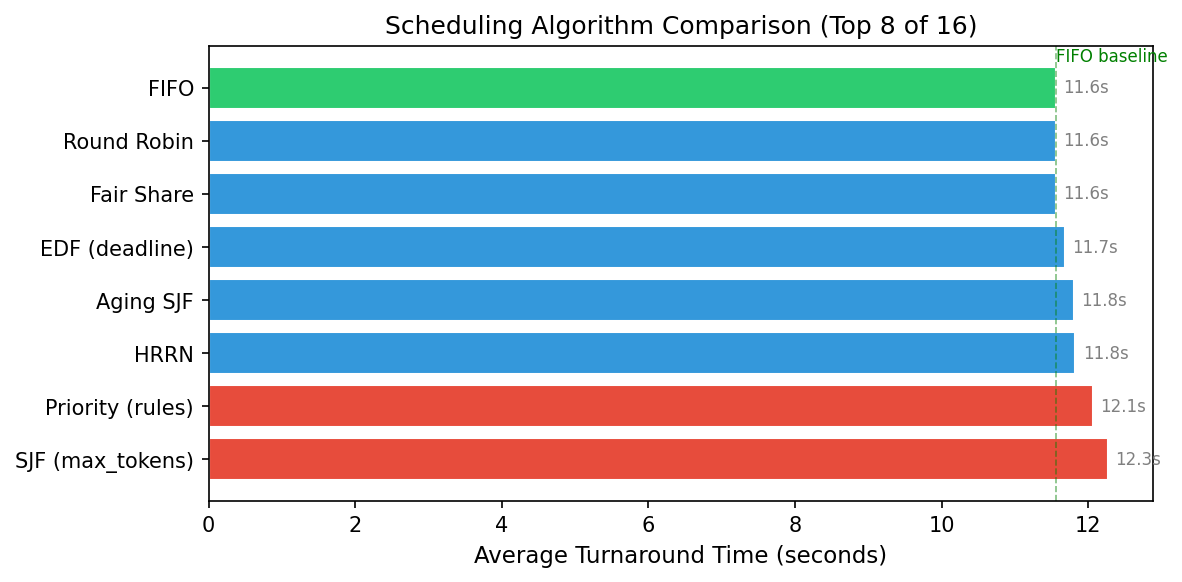
\includegraphics[width=\columnwidth]{algorithm_comparison_bar.png}}
\caption{Average turnaround time for top 8 of 16 simulated algorithms. FIFO (green) achieves the lowest turnaround. All reordering strategies perform equal or worse.}
\label{fig:simulation}
\end{figure}

\textbf{Key finding:} FIFO matches or outperforms all 16 algorithms on average turnaround time. This result is consistent across batch windows of 1s, 3s, and 5s. A Welch's $t$-test between FIFO and SJF per-request turnaround times yields $p = 0.06$, and bootstrap confidence intervals (1,000 resamples) for the mean turnaround difference overlap zero. Neither test reaches significance at $\alpha = 0.05$, confirming that reordering provides no reliable benefit.

\subsection{Per-Class Tradeoff: The Hidden Dimension}

While FIFO wins on average, the per-class analysis reveals a significant tradeoff that the overall metric obscures:

\begin{table}[htbp]
\caption{Per-Class Average Wait Time (ms) --- The Fairness Tradeoff}
\begin{center}
\begin{tabular}{lrrrl}
\toprule
\textbf{Algo.} & \textbf{Fast} & \textbf{Medium} & \textbf{Large} & \textbf{Tradeoff} \\
\midrule
FIFO & 5,400 & 5,385 & 6,223 & Uniform \\
SJF & 1,711 & 5,862 & 12,041 & $-$68\% fast, $+$94\% large \\
Priority & 1,447 & 6,577 & 10,931 & $-$73\% fast, $+$76\% large \\
\bottomrule
\end{tabular}
\label{tab:perclass}
\end{center}
\end{table}

SJF reduces fast-task wait by 68\% (5,400 $\rightarrow$ 1,711ms) at the cost of nearly doubling large-task wait (6,223 $\rightarrow$ 12,041ms). This tradeoff is meaningful: in systems where a QA chatbot requires sub-3-second responses while a background code generator can tolerate 15 seconds, Priority scheduling is strictly superior to FIFO.

\begin{figure}[htbp]
\centerline{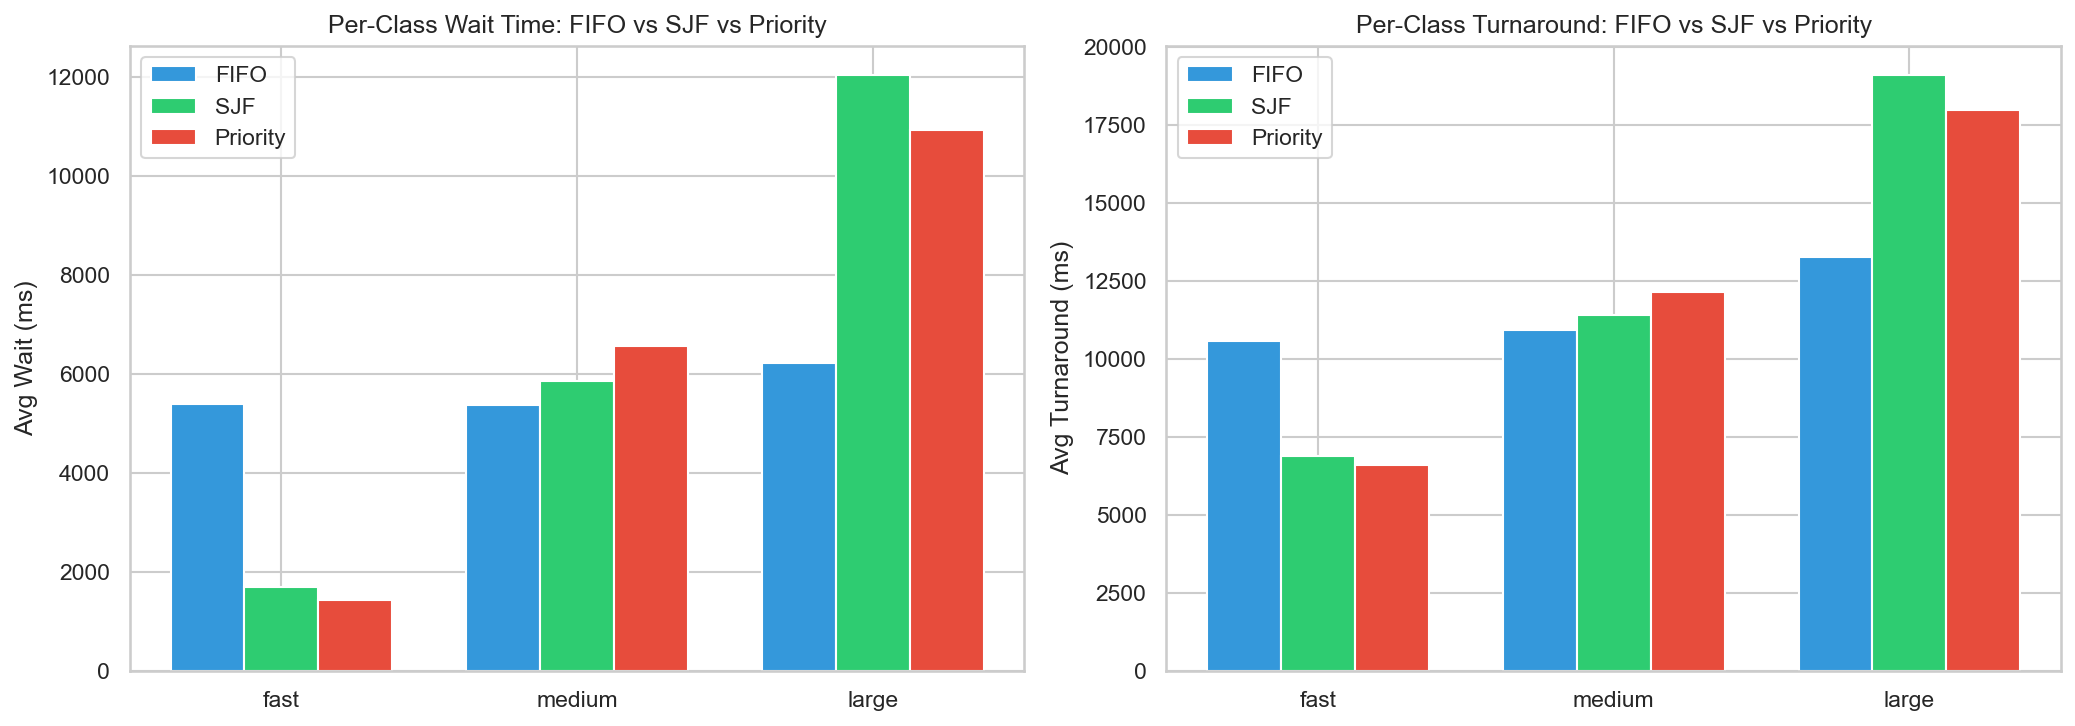
\includegraphics[width=\columnwidth]{perclass_comparison.png}}
\caption{Per-class wait and turnaround for FIFO vs SJF vs Priority. Priority-aware algorithms shift wait from fast to large tasks.}
\label{fig:perclass}
\end{figure}

% ============================================================
\section{Why FIFO Wins: A Theoretical Analysis}
\label{sec:why_fifo}
% ============================================================

The optimality of FIFO contradicts the classical result that SJF minimizes average waiting time~\cite{liu1973scheduling}. We identify two structural reasons.

\subsection{Violated Assumption 1: Job-Size Observability}

SJF requires knowing (or estimating) job completion time before execution. In classical OS scheduling, job size is either declared by the user or estimated from process metadata. For LLM requests, the relevant ``job size'' is the \textit{number of tokens the model will actually generate}---which depends on:

\begin{itemize}
    \item The semantic complexity of the prompt
    \item The model's internal state and sampling randomness
    \item The EOS token probability at each decode step
\end{itemize}

None of these are observable from request metadata. The \texttt{max\_tokens} parameter provides only a loose upper bound. In our dataset, the Spearman correlation between \texttt{max\_tokens} and \texttt{latency\_ms} is only $\rho = 0.206$, confirming that the ``job size'' is effectively hidden.

\subsection{Violated Assumption 2: Sequential Execution}

SJF's optimality proof assumes jobs execute one at a time. GPU-based LLM inference batches multiple requests: the prefill phase runs in parallel, and the decode phase is dominated by the longest-generating request in the batch. Formally, for a batch $B = \{r_1, \ldots, r_k\}$:

\begin{equation}
T_{\text{batch}} \approx T_{\text{prefill}}(B) + \max_{r_i \in B} T_{\text{decode}}(r_i)
\label{eq:batch}
\end{equation}

\begin{figure}[htbp]
\centering
\resizebox{\columnwidth}{!}{%
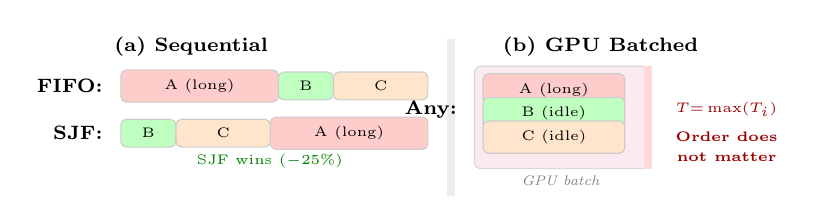
\begin{tikzpicture}[font=\scriptsize,
    req/.style={draw=gray!40, minimum height=0.35cm, anchor=west, rounded corners=2pt},
    lbl/.style={font=\scriptsize\bfseries}]
% Sequential
\node[lbl] at (1, 2.4) {(a) Sequential};
\node[lbl, anchor=east] at (0, 1.9) {FIFO:};
\node[req, fill=red!20, minimum width=2cm] at (0.1, 1.9) {\tiny A (long)};
\node[req, fill=green!25, minimum width=0.7cm] at (2.1, 1.9) {\tiny B};
\node[req, fill=orange!20, minimum width=1.2cm] at (2.8, 1.9) {\tiny C};
\node[lbl, anchor=east] at (0, 1.3) {SJF:};
\node[req, fill=green!25, minimum width=0.7cm] at (0.1, 1.3) {\tiny B};
\node[req, fill=orange!20, minimum width=1.2cm] at (0.8, 1.3) {\tiny C};
\node[req, fill=red!20, minimum width=2cm] at (2.0, 1.3) {\tiny A (long)};
\node[font=\tiny, green!50!black] at (2, 0.95) {SJF wins ($-$25\%)};
% Divider
\fill[gray!15] (4.25, 0.5) rectangle (4.35, 2.5);
% Batched
\node[lbl] at (6.2, 2.4) {(b) GPU Batched};
\node[lbl, anchor=east] at (4.5, 1.6) {Any:};
\fill[purple!8, rounded corners=2pt] (4.6, 0.85) rectangle (6.8, 2.15);
\draw[gray!30, rounded corners=2pt] (4.6, 0.85) rectangle (6.8, 2.15);
\node[req, fill=red!20, minimum width=1.8cm] at (4.7, 1.85) {\tiny A (long)};
\node[req, fill=green!25, minimum width=1.8cm] at (4.7, 1.55) {\tiny B (idle)};
\node[req, fill=orange!20, minimum width=1.8cm] at (4.7, 1.25) {\tiny C (idle)};
\node[font=\tiny, gray] at (5.7, 0.7) {\textit{GPU batch}};
\fill[red!15] (6.75, 0.85) rectangle (6.85, 2.15);
\node[font=\tiny, red!60!black, align=left] at (7.8, 1.6) {$T{=}\max(T_i)$};
\node[font=\tiny, red!60!black, align=left] at (7.8, 1.25) {\textbf{Order does}};
\node[font=\tiny, red!60!black, align=left] at (7.8, 1.0) {\textbf{not matter}};
\end{tikzpicture}%
}
\caption{Why SJF fails under GPU batching. (a)~Sequential: SJF reduces $\bar{T}$ by 25\%. (b)~Batched: all complete at $\max(T_i)$; reordering is ineffective.}
\label{fig:batching}
\end{figure}

Since the batch completion time is governed by the \textit{slowest} request (Eq.~\ref{eq:batch}), reordering within the batch does not change the total execution time. Fig.~\ref{fig:batching} illustrates this: under sequential execution, SJF reduces average turnaround by scheduling short jobs first; under batched execution, all jobs finish together, eliminating the benefit. This follows because SJF is provably optimal under sequential execution~\cite{silberschatz2018os}; therefore, any lack of improvement in this setting implies even weaker gains under coupled batch execution.

\subsection{Implication}
For batched LLM inference on a single GPU, the scheduling lever is \textit{batch composition} (which requests are grouped together), not \textit{dispatch order} (the sequence within a batch). This suggests that future work should focus on batch-aware scheduling rather than classical reordering algorithms.

% ============================================================
\section{Comparison with AIOS}
% ============================================================

Our results appear to contradict AIOS's finding that scheduling provides up to 2.1$\times$ throughput improvement~\cite{mei2025aios}. The difference is explained by what is being compared:

\begin{itemize}
    \item \textbf{AIOS result:} AIOS \textit{with} a scheduler vs. frameworks \textit{without} any scheduler (raw agent frameworks that flood the GPU and trigger CUDA OOM retries). The 2.1$\times$ improvement comes from \textit{having a scheduler at all}, not from the scheduling algorithm choice.
    \item \textbf{Our result:} FIFO vs. other algorithms, \textit{all within AIOS's scheduler framework}. Given that a scheduler exists, the choice of algorithm has minimal impact on average turnaround for single-GPU batched inference.
\end{itemize}

These results are complementary: \textbf{AIOS demonstrates the necessity of scheduling; our work demonstrates the limits of scheduling under GPU batching.} The gap between ``no scheduler'' and ``any scheduler'' is 2.1$\times$; the gap between FIFO and the best alternative is~$<$1\%.

% ============================================================
\section{Implementation}
% ============================================================

We implement six scheduler variants as drop-in replacements in the AIOS kernel, all extending \texttt{BaseScheduler}:

\begin{itemize}
    \item \texttt{fifo}: Original arrival-order dispatch (baseline).
    \item \texttt{sjf}: Sort batch by \texttt{max\_tokens} ascending.
    \item \texttt{priority}: Three-level queues (P0: \texttt{max\_tokens}$\leq$128; P1: $\leq$512 without tools; P2: rest) with aging promotion.
    \item \texttt{mlfq}: Dynamic demotion based on observed agent-type latency; periodic priority boost every 30s.
    \item \texttt{hrrn}: Response ratio = $(W + S)/S$ where $S$ = \texttt{max\_tokens}/100.
    \item \texttt{cognitive}: Trained Gradient Boosting classifier routing to fast/medium/large queues.
\end{itemize}

Selection requires a single config change (\texttt{scheduler\_type} in \texttt{config.yaml}). No code modification needed.

% ============================================================
\section{Discussion}
% ============================================================

\subsection{When Priority Scheduling is Justified}
Our simulation shows FIFO wins on average but loses on \textit{fairness}. In systems with heterogeneous latency SLAs---e.g., a real-time assistant agent requiring $<$3s response alongside a batch code-generation agent tolerating 15s---Priority scheduling reduces the assistant's wait by 73\% at an acceptable cost to the batch agent. The choice between FIFO and Priority is thus an \textit{engineering decision} driven by deployment requirements, not a universal optimum.

\subsection{Limitations}
\begin{itemize}
    \item \textbf{Single inference backend:} Multi-GPU setups with model parallelism or request routing may exhibit different dynamics.
    \item \textbf{Similar model sizes:} 7B vs 8B parameters produce only 920ms median difference. Larger gaps (e.g., 7B vs 70B) would amplify model-name as a feature.
    \item \textbf{Sequential simulation:} Our simulation does not model GPU batching directly. The sequential model provides an upper bound on reordering benefit---if reordering provides no improvement under sequential execution (where it theoretically should help most), it will provide even less under batched execution. A batch-level simulator modeling GPU kernel execution and token-level synchronization is beyond scope but represents important future work.
    \item \textbf{No preemptive algorithms:} AIOS supports Round Robin with context interruption, but we evaluate only non-preemptive strategies.
    \item \textbf{Dataset size:} 2,000 syscalls provides sufficient coverage for our controlled parameter space but may not generalize to production workloads with open-ended prompt distributions.
\end{itemize}

\subsection{Future Work}
\begin{itemize}
    \item \textbf{Live batch-composition experiments}: Deploy SJF and Priority on the live AIOS kernel to test whether separating fast and slow requests into different batches yields improvement beyond what simulation predicts.
    \item \textbf{Output length prediction}: A lightweight model predicting \textit{actual} generation length (rather than the budget ceiling) could restore SJF's theoretical advantage.
    \item \textbf{Multi-GPU scheduling}: With heterogeneous models across GPUs, request-aware routing becomes a load-balancing problem with richer optimization potential.
    \item \textbf{RL-based adaptive scheduling}: A reinforcement learning agent that optimizes dispatch policy from reward signals (latency, throughput, fairness) could discover non-obvious strategies.
\end{itemize}

% ============================================================
\section{Conclusion}
% ============================================================

We investigated whether classical OS scheduling assumptions hold for LLM agent systems and found they do not. Our three-phase study on 2,000 AIOS syscalls across two LLM backends reveals:

\begin{enumerate}
    \item \textbf{Job-size observability fails:} Request features are weak latency predictors (max $\rho = 0.206$) because \texttt{max\_tokens} is a ceiling and actual output length is unobservable.
    \item \textbf{ML cannot bridge the gap:} The best classifier achieves F1 = 0.47, confirming that the feature space does not cleanly partition into latency classes.
    \item \textbf{FIFO is near-optimal:} Among 16 simulated algorithms, no strategy reduces average turnaround below FIFO, because GPU batching nullifies SJF's sequential-execution assumption.
    \item \textbf{A fairness tradeoff exists:} SJF and Priority reduce fast-task wait by 68--73\% at the cost of large-task degradation---a dimension the original AIOS design does not address.
\end{enumerate}

These findings suggest that the scheduling frontier for LLM agent systems lies not in dispatch order but in \textit{batch composition}---deciding which requests to group for GPU execution. We release our instrumented kernel, six scheduler implementations, and simulation framework to enable future research at this intersection of operating systems and LLM infrastructure.

\section*{Acknowledgment}
This work builds upon the AIOS architecture by Mei et al.~\cite{mei2025aios} at Rutgers University. We thank the AIOS team for their open-source codebase and the Ollama project for accessible local LLM inference.

\begin{thebibliography}{00}
\bibitem{mei2025aios} K.~Mei \textit{et al.}, ``AIOS: LLM agent operating system,'' in \textit{Proc. COLM}, 2025.
\bibitem{ge2023llm} Y.~Ge \textit{et al.}, ``LLM as OS, agents as apps: Envisioning AIOS, agents and the AIOS-agent ecosystem,'' \textit{arXiv:2312.03815}, 2023.
\bibitem{yao2023react} S.~Yao \textit{et al.}, ``ReAct: Synergizing reasoning and acting in language models,'' in \textit{Proc. ICLR}, 2023.
\bibitem{shinn2023reflexion} N.~Shinn \textit{et al.}, ``Reflexion: Language agents with verbal reinforcement learning,'' in \textit{Proc. NeurIPS}, 2023.
\bibitem{rama2025cerebrum} B.~Rama, K.~Mei, and Y.~Zhang, ``Cerebrum (AIOS SDK),'' in \textit{Proc. NAACL}, 2025.
\bibitem{packer2023memgpt} C.~Packer \textit{et al.}, ``MemGPT: Towards LLMs as operating systems,'' \textit{arXiv:2310.08560}, 2023.
\bibitem{silberschatz2018os} A.~Silberschatz, P.~B.~Galvin, and G.~Gagne, \textit{Operating System Concepts}, 10th~ed. Wiley, 2018.
\bibitem{liu1973scheduling} C.~L.~Liu and J.~W.~Layland, ``Scheduling algorithms for multiprogramming in a hard-real-time environment,'' \textit{J.~ACM}, vol.~20, no.~1, pp.~46--61, 1973.
\bibitem{corbato1962experimental} F.~J.~Corbat\'{o}, M.~Merwin-Daggett, and R.~C.~Daley, ``An experimental time-sharing system,'' in \textit{Proc. AFIPS}, 1962, pp.~335--344.
\bibitem{kraska2018case} T.~Kraska \textit{et al.}, ``The case for learned index structures,'' in \textit{Proc. SIGMOD}, 2018.
\bibitem{mao2019learning} H.~Mao \textit{et al.}, ``Learning scheduling algorithms for data processing clusters,'' in \textit{Proc. SIGCOMM}, 2019.
\bibitem{chen2018tvm} T.~Chen \textit{et al.}, ``TVM: An automated end-to-end optimizing compiler for deep learning,'' in \textit{Proc. OSDI}, 2018.
\bibitem{sheng2023flexgen} Y.~Sheng \textit{et al.}, ``FlexGen: High-throughput generative inference of large language models with a single GPU,'' in \textit{Proc. ICML}, 2023.
\bibitem{ollama} ``Ollama,'' \url{https://ollama.com}, 2024.
\bibitem{dubey2024llama} A.~Dubey \textit{et al.}, ``The Llama 3 herd of models,'' \textit{arXiv:2407.21783}, 2024.
\bibitem{jiang2023mistral} A.~Q.~Jiang \textit{et al.}, ``Mistral 7B,'' \textit{arXiv:2310.06825}, 2023.
\end{thebibliography}

\end{document}
